% \documentclass{article}
\documentclass[tikz,margin=5mm]{standalone}
\usepackage{tikz}
\usetikzlibrary{arrows.meta}
\begin{document}
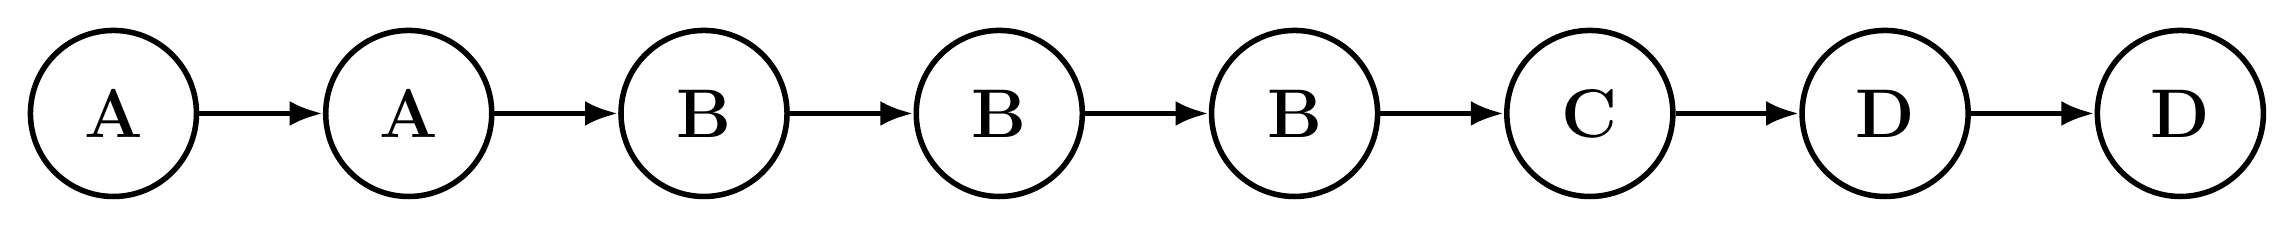
\begin{tikzpicture}[
  scale=2.5,
  every node/.style = {minimum width = 6em, draw, circle, font=\Huge\bf, line width=2pt, scale=1},
  edge from parent/.style={-{Latex}, line width=2pt, draw},
  level/.style = {sibling distance = 60mm/#1}
]
  \node {A}
    child[grow=right] {
        node {A}  
        child [grow=right]{
          node {B}
          child [grow=right]{
            node {B}
            child [grow=right]{
              node {B}
              child [grow=right]{
                node {C}
                child [grow=right]{
                  node {D}
                  child [grow=right]{
                    node {D}
      }}}}}}};
\end{tikzpicture}
\end{document}

